\documentclass{mycv}

\newboolean{GERMAN_CV}\setboolean{GERMAN_CV}{false}


\newcommand{\CVRole}{senior software engineer}
\newcommand{\CVFields}{autonomous driving, machine learning and artificial intelligence}


\begin{document}
\sloppy % this restricts words spilling out of the margins
\color{templateColor1}
\pagenumbering{gobble}
% \AddToShipoutPicture{\BackgroundPic}

\normalfont
\begin{minipage}[]{0.68\textwidth}
    \vspace{5mm}

    {\huge Dr.-Ing. }\\

    {\Huge Chandramouli}\\

    {\Huge Gnanasambandham}
    \vspace{2mm}

    \vspace{2mm}

    {\large
        Steinweg 24\\
        71263 Weil der Stadt\\

        \ifthenelse{\boolean{GERMAN_CV}}
        {
            \dateOfBirthIcon 6. August 1990\\
        }
        {
            \dateOfBirthIcon 6\textsuperscript{th} August 1990\\
        }
        \telephoneIcon +49 179 6588043\\
        \mailIcon \href{mailto:chandramouli681990@gmail.com}{\link{chandramouli681990@gmail.com}}
    }
  
    \vspace{13mm}
\end{minipage}
\begin{minipage}[c]{0.32\textwidth}
    %\centering
  %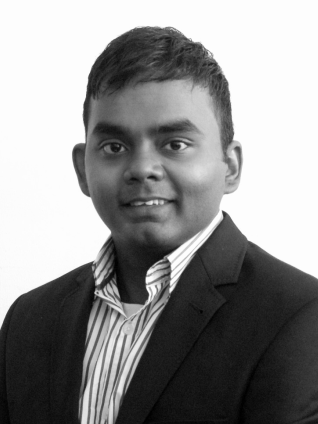
\includegraphics[width=5.2cm]{../img/CV_Photo_comp.png}
  %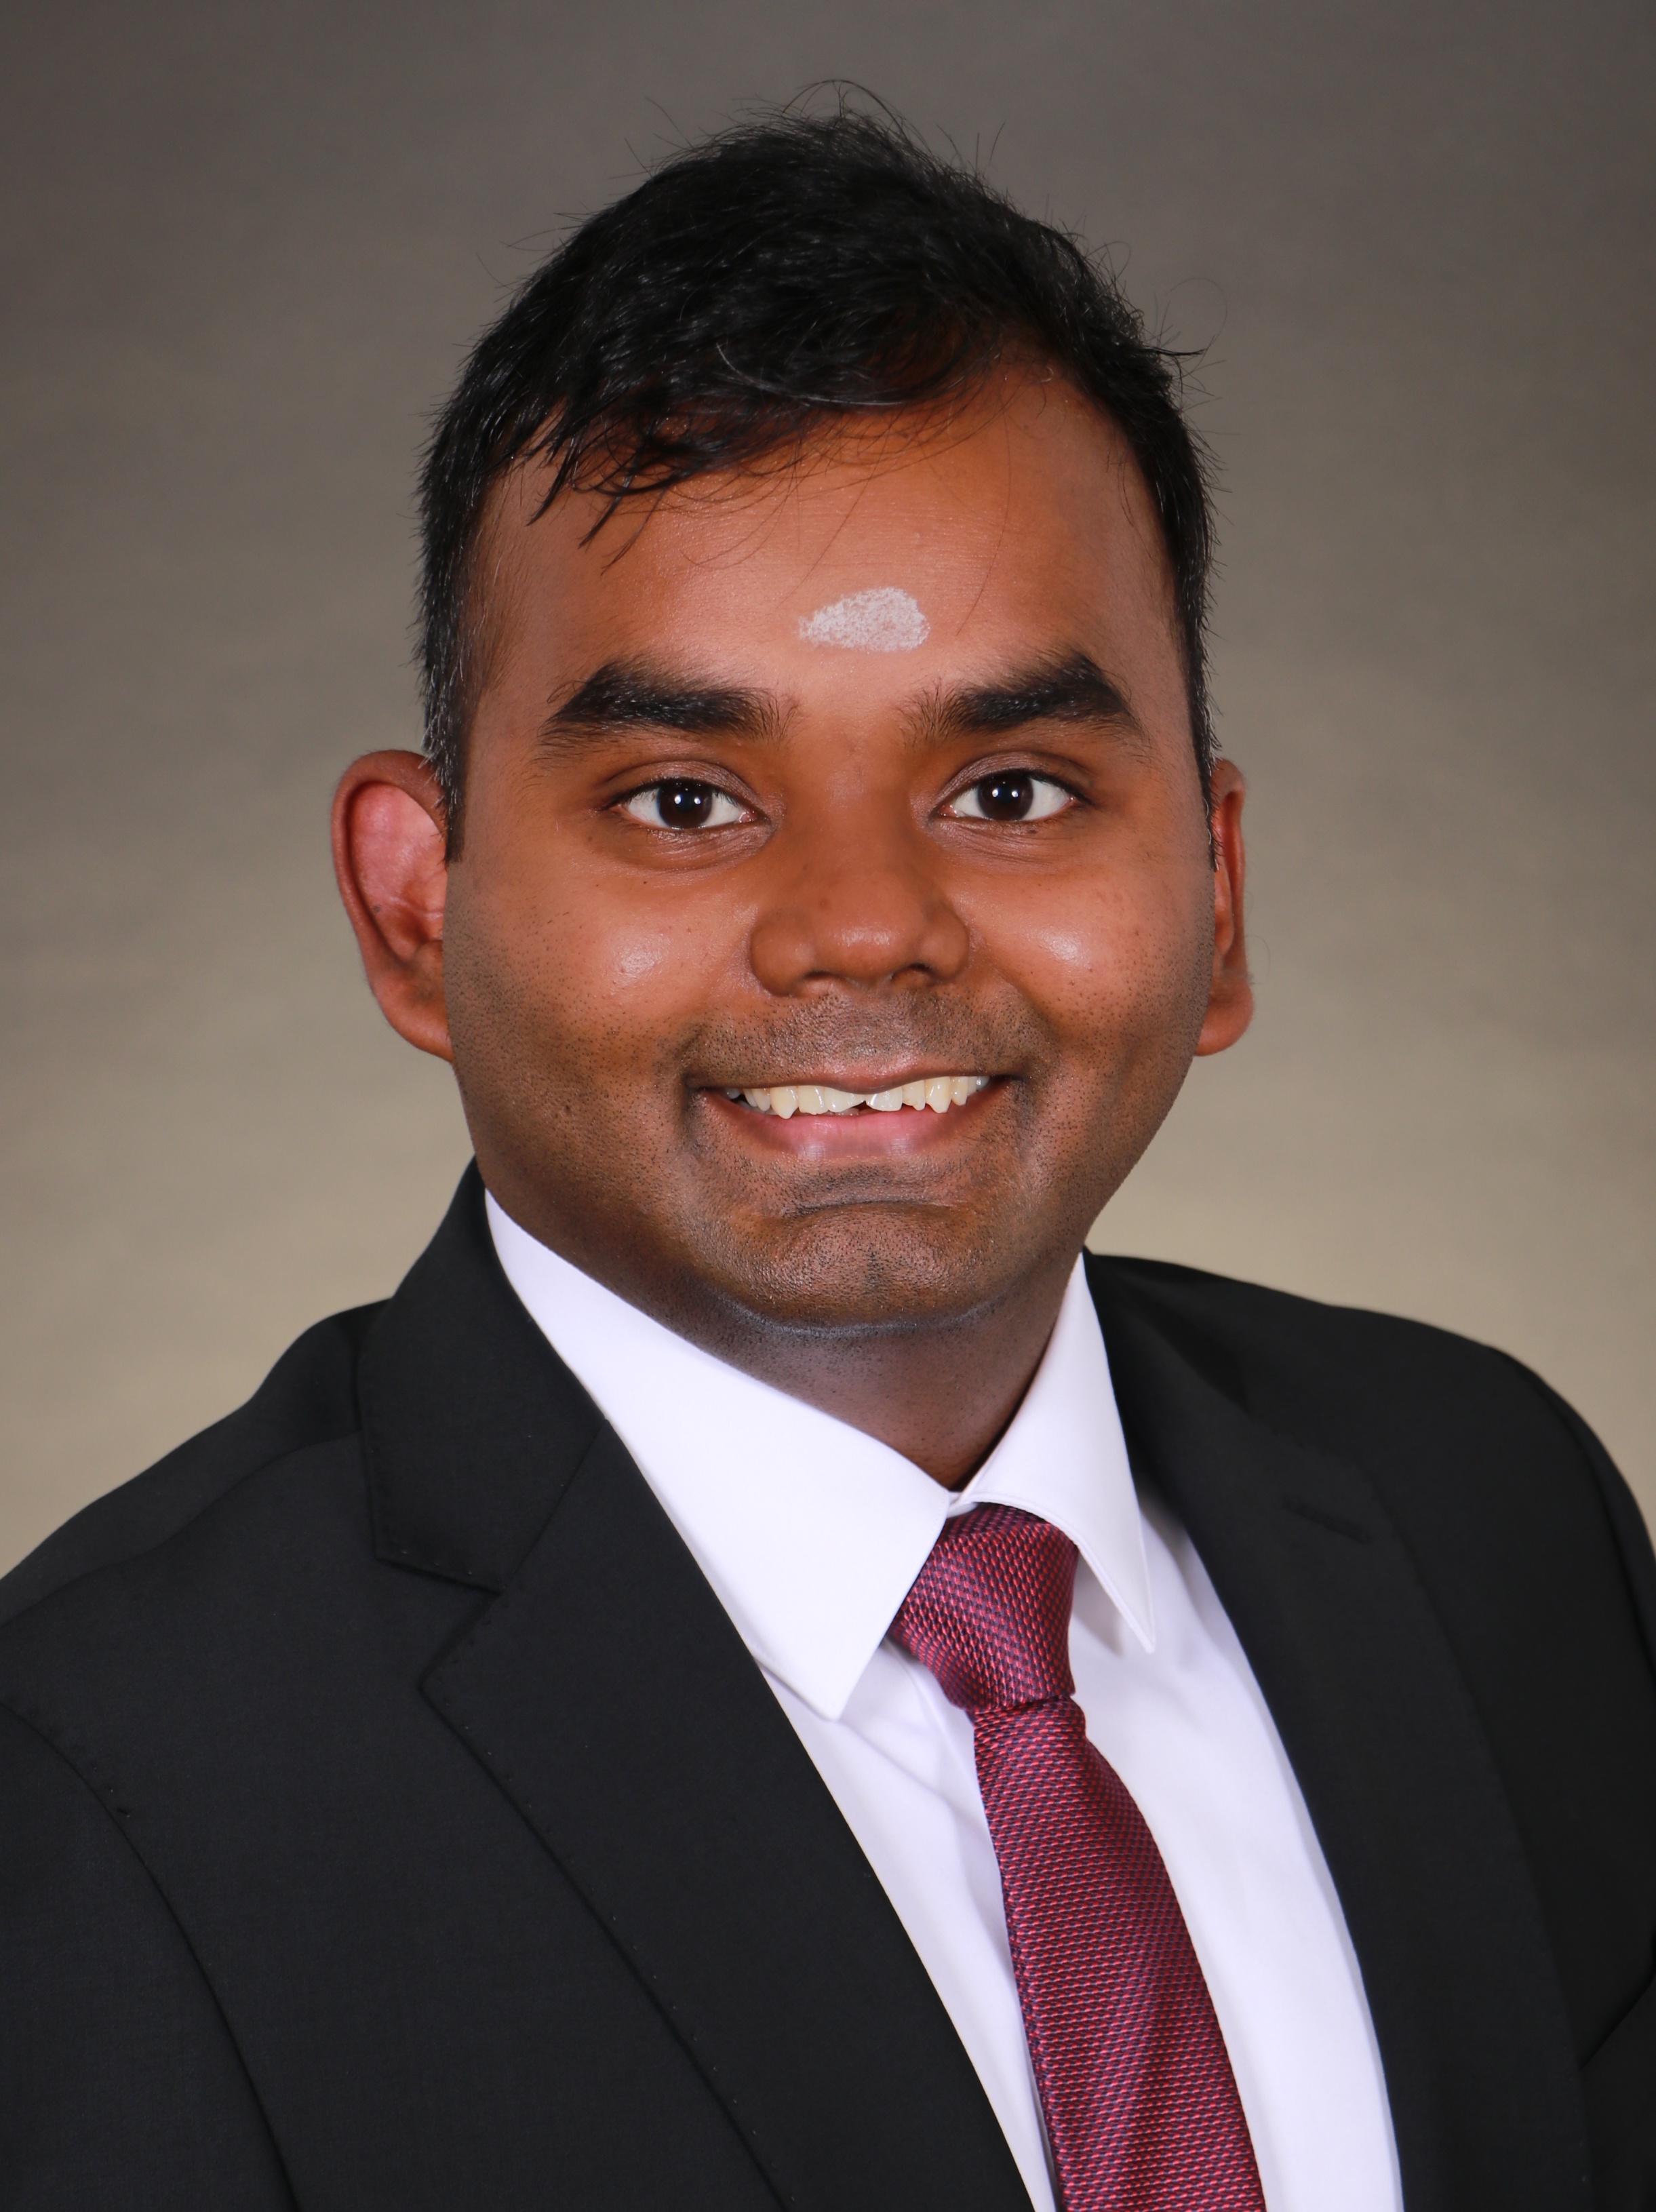
\includegraphics[width=5.45cm]{../img/IMG_7896_m02.jpg}
  % 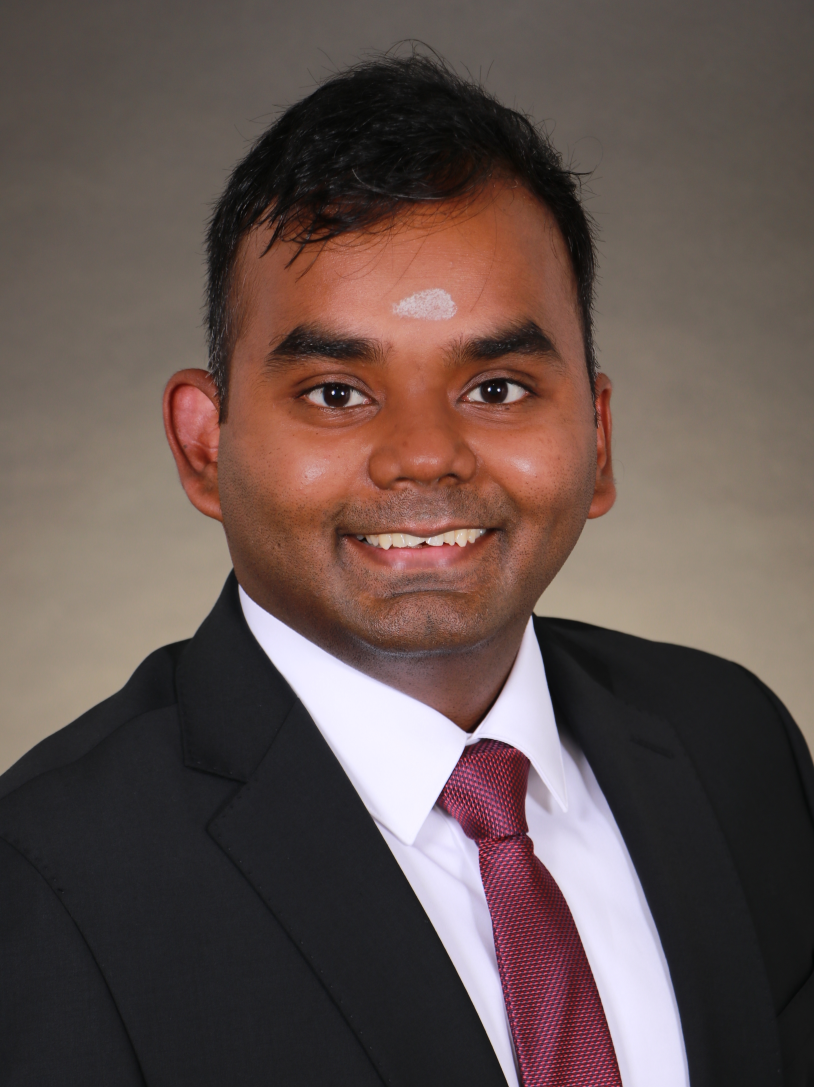
\includegraphics[width=5.45cm]{../img/CV_Photo_new_comp.png}
  % 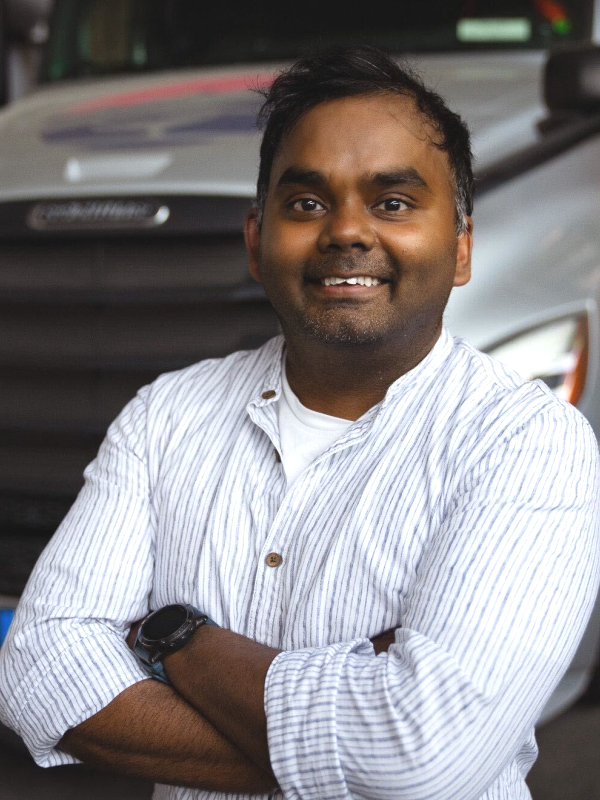
\includegraphics[width=5.7cm]{../img/CV_Photo_Informal_Comp.png}
  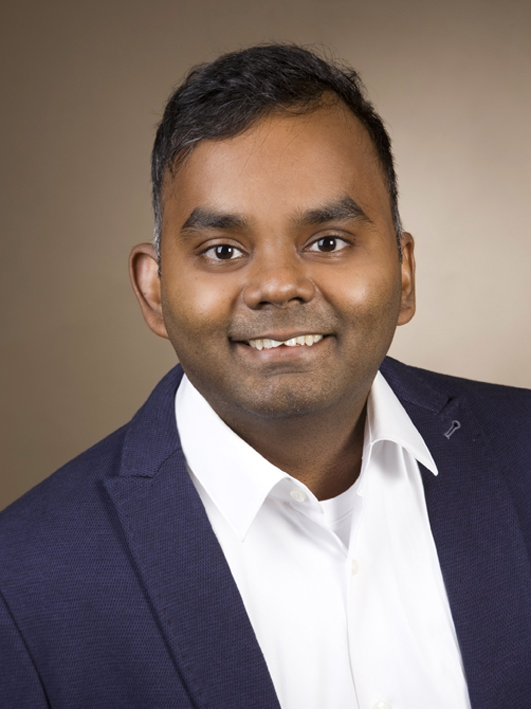
\includegraphics[width=5.5cm]{../img/ChandramouliNew1.jpg}
\end{minipage}

{\rlap{\color{templateColor4}\rule[0mm]{\textwidth}{\ulinewidth}}}
\columnratio{0.39}
\setlength{\columnsep}{2.5em}
\setlength{\columnseprule}{\ulinewidth}
\colseprulecolor{templateColor4}
\begin{paracol}{2}
    \ifthenelse{\boolean{GERMAN_CV}}
    {
        \lsection{Profil}

        Ich bin ein leidenschaftlich neugieriger Ingenieur mit hervorragenden
        interkulturellen Kommunikationsf{\"a}higkeiten. Aktuell leite ich die
        Entwicklung robuster Fahrzeugmodelle für hochskalierbare Simulationen,
        mit mehr als 200 aktiven Nutzern. Die Abstimmung mit
        interdisziplin{\"a}ren, internationalen Nutzern findet {\"u}ber
        verschiedene Zeitzone hinweg. Während meiner Zeit an der Universität
        war ich Erstautor von 6 Artikeln in renommierten Fachzeitschriften im
        Bereich Partikeldynamik, verfasst mit führenden Wissenschaftsexperten.
        All dies wurde durch meine Anpassungsfähigkeit sowie herausragende
        analytische und Teamfähigkeiten ermöglicht. Jetzt strebe ich eine neue
        Herausforderung als Senior Engineer an, um meine Expertise in
        Simulation in innovative Mobilit{\"a}tsl{\"o}sungen einzubringen.\\

    } 
    { 

        \lsection{Profile}

        I am a passionately curious engineer with excellent intercultural
        communication skills. I have been spearheading the development of
        robust multi-fidelity vehicle models for highly-scalable simulations
        with over 300 active users in my current organization. Coordination
        with interdisciplinary, international users takes place across
        different time zones. Moreover, I have been first author of 6
        peer-reviewed journal articles in particle dynamics during my time at
        the academia, collaborating closely with leading scientific minds. All
        this was possible, thanks to my exceptional adaptability to rapidly
        changing environments and my extraordinary analytical and team skills.
        I am now seeking new opportunities as a Senior 
        Engineer, where I can leverage my expertise in simulation to contribute
        to cutting-edge innovations in aerospace.\\

    }

  \ifthenelse{\boolean{GERMAN_CV}}
  {
      \lsection{Sprachen}
      \begin{onehalfspace}
      \begin{tabular}{
                p{2cm} >{\raggedleft\arraybackslash}p{4.5cm}}
                {\mybox\mybox\mybox\mybox\mybox}  & {flie{\ss}end| Deutsch} \\
                {\mybox\mybox\mybox\mybox\mybox} & {flie{\ss}end | Englisch}\\
                {\mybox\mybox\mybox\mybox\mybox}  & {Muttersprache | Tamil}  \\
                {\mybox\mybox\mybox\mybox\myboxo}  & {fortgeschritten | Hindi}\\\\
      \end{tabular}
      \end{onehalfspace}
  }
  {

      \lsection{Languages}
      \begin{onehalfspace}
          \begin{tabular}{
                  p{2cm} >{\raggedleft\arraybackslash}p{4.5cm}}
                  {\mybox\mybox\mybox\mybox\mybox}  & {Proficient | German} \\
                  {\mybox\mybox\mybox\mybox\mybox} & {Proficient | English}\\
                  {\mybox\mybox\mybox\mybox\mybox}  & {Mother tounge | Tamil}  \\
                  {\mybox\mybox\mybox\mybox\myboxo}  & {Advanced | Hindi}\\\\
          \end{tabular}
      \end{onehalfspace}
  }

        \lsection{Web}
        \begin{minipage}[c]{0.31\textwidth}
            \begin{flushright}
                {\bfseries Linkedin}\\
                {\footnotesize
                    \href{https://linkedin.com/in/gnanasambandhamc}{\link{linkedin.com/in/gnanasambandhamc}}}
            \end{flushright}
        \end{minipage}
        \begin{minipage}{0.05\textwidth}
            \linkedinIcon
        \end{minipage}
        \vspace{3mm}

        \begin{minipage}[c]{0.31\textwidth}
            \begin{flushright}
                {\bfseries GitHub}\\
                {\footnotesize \href{https://github.com/chandramouli6890/}{\link{github.com/chandramouli6890}}}
            \end{flushright}
        \end{minipage}
        \begin{minipage}{0.05\textwidth}
            \githubIcon
        \end{minipage}
        \vspace{3mm}

        % \begin{minipage}[c]{0.31\textwidth}
        %     \begin{flushright}
        %         {\bfseries Medium}\\
        %         {\footnotesize \href{https://chandramoulig.medium.com}{\link{chandramoulig.medium.com}}}
        %     \end{flushright}
        % \end{minipage}
        % \begin{minipage}{0.05\textwidth}
        %     \mediumIcon
        % \end{minipage}
        % \vspace{3mm}

        \begin{minipage}[c]{0.31\textwidth}
            \begin{flushright}
                {\bfseries Matlab}\\
                {\footnotesize
                    \href{https://de.mathworks.com/matlabcentral/profile/authors/4267772}{\link{MatlabCentral    Profile}}}
            \end{flushright}
        \end{minipage}
        \begin{minipage}{0.05\textwidth}
            \matlabIcon
        \end{minipage}

\switchcolumn

\ifthenelse{\boolean{GERMAN_CV}}
{
    \rsection{Beruflicher Werdegang}
    \subsection{04/2023 - 03/2025}{Torc Europe GmbH, Stuttgart}{\bfseries Staff Software Engineer}
          \begin{itemize}

            \item Leitung eines Teams zur Entwicklung eines skalierbaren
                Fahrzeugmodells in C++ mit Test-Driven Development (TDD) und
                objektorientierter Programmierung (OOP).

            \item Integration von Fahrzeugmodellen mit unterschiedlichem
                Detailierungsgrad in einen ROS-basierten Simulator zur
                virtuellen Validierung von Level-4 autonomen LKWs.
            
            \item Modellierung meschanischer Bauteile (Reifen, Lenkung),
                Steuerger{\"a}ten (Lenkung, Schaltung).

            \item Umsetzung von hohen numerischen und softwaretechnischen
                Entwickulngsstandards. 

            \item Zusammenarbeit mit externen Partnern, um eine skalierbare
                Qualifizierungsstrategie für Fahrzeugmodelle gem{\"a}{\ss} den
                ISO-26262 zu entwickeln.

          \end{itemize}
     
          \subsection{08/2021 - 03/2023}{Daimler Truck AG, Stuttgart}{{\bfseries Entwicklungsingenieur}}
           \begin{itemize}
               \item Entwicklung von Fahrzeugmodelle mit unterschiedlichem
                   Detailierungsgrad f{\"u}r skalierbare Simulationen in MATLAB/Simulink.

               \item Entwicklung einer C++ Co-Simulations-Schnittstelle zur
                   Kopplung eines hochdetaillierten Mehrk{\"o}rpermodells mit
                   einem virtuellen Fahrer für hochdynamischen
                   Man{\"o}versimulationen.
           \end{itemize}

        \subsection{05/2016 - 04/2021}{Universit{\"a}t
            Stuttgart}{{\bfseries Wissenschaftlicher Mitarbeiter}}
           \begin{itemize}
               \item Entwicklung \& Administration der Partikelsimulationssoftware
                   Pasimodo in C++.
               \item Planung und Durchf{\"u}hrung von Analysen
                   schwingungsbehafteter Systeme mit Laser-Doppler Vibrometer.
               \item Organisation und Durchf{\"u}hrung von Veranstaltungen f{\"u}r
                   die Vorlesung "Fahrzeugdunamik" und Durchf{\"u}hrung von
                   Laborpraktika.
           \end{itemize}

        \subsection{10/2015 - 04/2016}{Fraunhofer Institute (ITWM), Kaiserslautern}
            {{\bfseries Werkstudent}}\\
}
{
    \rsection{Professional Career}
    \subsection{04/2023 - present}{Torc Europe GmbH, Stuttgart}{{\bfseries Staff Software Engineer}}
          \begin{itemize}
            \item Spearheaded a team to develop a highly-scalable
                vehicle model in C++ following Test-Driven Development
                (TDD) and Object-Oriented Programming (OOP).
            \item Integrated vehicle models into a Robotic Operating System (ROS)
                based simulator to enable virtual validation of Level 4
                autonomous vehicles.
            \item Communication and presentation of team results to senior management and within the company.
            \item Scripting for auto-generating documentation from code based on Git-events.
            \item Collaborated with external stakeholders to develop a scalable
                validation strategy for vehicle models as per ISO-26262.
          \end{itemize}
    
    \subsection{08/2021 - 03/2023}{Daimler Truck AG, Stuttgart}{\bfseries Vehicle model engineer}
          \begin{itemize}
              \item Develop multi-fidelity vehicle models for scalable simulations in the context of
          virtual validation in MATLAB/Simulink
            \item Developed a co-simulation interface in C++ to couple a high-fidelity
                multibody truck model and the virtual driver using
                TCP/IP communication interface.
          \end{itemize}

    \subsection{05/2016 - 04/2021}{University of Stuttgart}{{\bfseries Scientific Staff}}
           \begin{itemize}
               \item Development and administration of the particle simulation
                   software Pasimodo in C++.
               \item Planning and execution of measurement campaigns of
                   virbational structures using Laser-Doppler Vibrometry.
               \item Organisation und assistance for the lecture "Vehicle
                   Dynamics" and supervision of lab workshops
           \end{itemize}

    \subsection{10/2015 - 04/2016}{Fraunhofer Institute (ITWM), Kaiserslautern}
        {{\bfseries Intern}}\\
}
\end{paracol}

{\rlap{\color{templateColor4}\rule[0mm]{\textwidth}{\ulinewidth}}}
\begin{paracol}{2}
    \switchcolumn
    \ifthenelse{\boolean{GERMAN_CV}}
    {
        \rsection{Ausbildung}
            \subsection{05/2016 - 04/2021}{\bfseries Dr.-Ing.}{\bfseries Universit{\"a}t
            Stuttgart}{in Maschinenbau (Note: magna cum laude)}
              \begin{itemize}
                  \item Dissertationstitel: \textit{Particle Dampers - Enhancing
                      Energy Dissipation using Fluid/Solid Interactions and Rigid
                  Obstacle-Grids}
              \end{itemize}
            
              \subsection{10/2012 - 04/2016}{{\bfseries M.Sc.} in Commercial
            Vehicle Tech. (Note: 1.9)}{\bfseries Technische Universit{\"a}t Kaiserslautern
            }\\
            
            \subsection{06/2008 - 04/2012}{{\bfseries B.Eng.} in
            Fertigunstechnik (Note:
            8.3/10 {sehr gut})} {\bfseries Anna University, Chennai, Indien }\\
    
    }
    {
        \rsection{Educational Qualification}
            \subsection{05/2016 -04/2021}
            {{\bfseries Ph.D.} in Mech. Eng. (Grade: magna cum laude)}
            {\bfseries University of Stuttgart}
              \begin{itemize}
                  \item Dissertation Titel: Particle Dampers - Enhancing
                      Energy Dissipation using Fluid/Solid Interactions and Rigid
                      Obstacle-Grids
              \end{itemize}
    
            \subsection{10/2012 - 04/2016}
            {{\bfseries M.Sc.} in Commercial Vehicle Tech. (Grade: 1.9)}
            {\bfseries Technical University of Kaiserslautern}\\
    
            \subsection{06/2008 - 04/2012}{{\bfseries B.Eng.} in
                Production Eng. (Grade: 8.3/10)}{\bfseries Anna University, Chennai, India}}\\
    }
    
    \ifthenelse{\boolean{GERMAN_CV}}
    {
        \rsection{Technische Qualifikationen}
        \begin{onehalfspace}
            \begin{tabular}{p{5cm}!{\color{templateColor1}\vrule}p{6.5cm}}
            {\bfseries Programmiersprachen: } & {\bfseries Betriebssystem:}\\
            {\mybox\mybox\mybox\mybox\mybox 12 Jahre | C/C++}  &
            {\mybox\mybox\mybox\mybox\mybox Linux (Debian, Ubuntu)}\\
            {\mybox\mybox\mybox\mybox\mybox 12 Jahre | MATLAB} & 
            {\mybox\mybox\mybox\mybox\myboxo Microsoft Windows}\\
            {\mybox\mybox\mybox\mybox\myboxo 9 Jahre | BASH}  & \\
            {\mybox\mybox\mybox\myboxo\myboxo 6 Jahre | Python}  & \\
        \end{tabular}\vspace{4mm}
        \end{onehalfspace}
    }
    {
        \rsection{Technical Skills}
        \begin{onehalfspace}
            \begin{tabular}{p{5cm}!{\color{templateColor1}\vrule}p{6.5cm}}
            {\bfseries Programming Languages: } & {\bfseries Operating System:}\\
            {\mybox\mybox\mybox\mybox\mybox 12 years | C/C++}  &
            {\mybox\mybox\mybox\mybox\mybox Linux (Debian, Ubuntu)}\\
            {\mybox\mybox\mybox\mybox\mybox 12 years | MATLAB} & 
            {\mybox\mybox\mybox\mybox\myboxo Microsoft Windows}\\
            {\mybox\mybox\mybox\mybox\myboxo 9 years | BASH}  & \\
            {\mybox\mybox\mybox\myboxo\myboxo 6 years | Python}  & \\
        \end{tabular}\vspace{4mm}
        \end{onehalfspace}
    }

    \ifthenelse{\boolean{GERMAN_CV}}
    {
        {\bfseries Prgramm-Kenntnisse:}
        \begin{itemize}
            \item {\bfseries MATLAB/Simulink:} Modellierung, Simulation,
                Optimierung, SiL/DiL simulations, MATLAB GUI, FMI
            \item {\bfseries C/C++:} MEX API, SilverBypass, FMI, ROS, TCP/IP and UDP
            \item{\bfseries Mehrk{\"o}rpersimulation:}  LMS Virtual.Lab Motion, Neweul-M$^2$, 
                MSC Adams, Project Chrono
            \item{\bfseries ADAS/AD-Simulationen:} Applied Object-Sim, IPG CarMaker
            \item {\bfseries sonstige Programme:}  Silver Virtual-ECU, COMSOL
                Multiphysics, OptiSlang, Oracle VM VirtualBox
        \end{itemize} \par

        {\bfseries Software Entwicklung:}\par
        \begin{itemize}
            \item {\bfseries Continuous Integration:} Git, GitHub Actions, Jenkins, Docker\par
            \item {\bfseries Testumgebungen:} {\verb|pytest}, Google test\par
            \item {\bfseries Technologien:} PETSc, EIGEN, OpenGL\par
            \item {\bfseries Debuggers/Profilers:} {\verb|gdb}, {\verb|valgrind}, {\verb|calgrind},
                Intel VTune
        \end{itemize}
    }
    {
        {\bfseries Simulation and Data Skills:}
        \begin{itemize}
            \item {\bfseries MATLAB/Simulink:} Modelling, \,simulation,
                numerical optimization, SiL/DiL simulations, MATLAB GUI, FMI
            \item {\bfseries C/C++:} MEX API, SilverBypass, FMI, ROS, TCP/IP and UDP
            \item{\bfseries Multibody-Simulation:}  LMS Virtual.Lab Motion, Neweul-M$^2$, 
                MSC Adams, Project Chrono
            \item{\bfseries ADAS/AD-Simulation Tools:}  Applied Object-Sim, IPG CarMaker
            \item{\bfseries Multibody-Simulation:}  LMS Virtual.Lab Motion, Neweul-M$^2$
            \item {\bfseries Other Software Tools:}  Silver Virtual-ECU, COMSOL
                Multiphysics, OptiSlang, Oracle VM VirtualBox
        \end{itemize} \par

        {\bfseries Software Development Tools:}\par
        \begin{itemize}
            \item {\bfseries CI Tools:} Git, GitHub Actions, Jenkins, Docker\par
            \item {\bfseries Testing Frameworks:} {\verb|pytest}, Google test\par
            \item {\bfseries Technologies:} PETSc, EIGEN, OpenGL\par
            \item {\bfseries Debuggers/Profilers:} {\verb|gdb}, {\verb|valgrind}, {\verb|calgrind},
                Intel VTune
        \end{itemize}
    }

\switchcolumn
\ifthenelse{\boolean{GERMAN_CV}}
{
    \lsection{Preise}
    {\RaggedLeft \bfseries Best Presentation Award 2014\\}
    Optimization of Vehicle Parameters based on Lap-Time
    Simulations using Multiobjective Evolutionary Algorithm\\

    {\RaggedLeft \bfseries Best Presentation Award 2015\\} An Adaptive
    Approach to Real-Time Estimation of Vehicle Dynamics Parameters using
    Kalman Filtering\\\\ 

    \lsection{Sonstige Projekte} 

    {\RaggedLeft 07/2020 - heute\\ \bfseries Raspberry Pi gesteuerte
    Smart-Home\\} Im Rahmen eines laufenden Hobbyprojekts habe ich ein
    vielseitiges Raspberry-Pi-Smart-Home-Netzwerk aufgebaut. Es umfasst
    Remote-SSH-Zugriff, einen flexiblen Datenserver mit
    automatischen Backups {\"u}ber {\verb|rsync}, einen Zigbee2Mqtt-Server zur
    Steuerung von IoT-Geräten z.B. über Siri.\\

    {\RaggedLeft 06/2015\\ \bfseries Machine Learning Suite\\} 
    Implementierung eines Deep-Convolution-Neural-Networks zur optischen
    Zeichenerkennung im Rahmen eines freiberuflichen Softwareprojekts in
    MATLAB. Zur Leistungssteigerung wurde die {MEX-API} genutzt. \\

    {\RaggedLeft 06/2014\\ \bfseries Driver-in-the-Loop Simulator\\} 
    Im Rahmen meiner Arbeit für ein Formula-Student-Rennteam entwickelte ich
    einen Driver-in-the-Loop-Simulator auf Basis einer
    Kommunikationsschnittstelle zwischen IPG CarMaker und MATLAB/Simulink.\\
}
{ 
    \lsection{Awards}
    {\RaggedLeft \bfseries Best Presentation Award 2014\\}
    Optimization of Vehicle Parameters based on Lap-Time
    Simulations using Multiobjective Evolutionary Algorithm\\

    {\RaggedLeft \bfseries Best Presentation Award 2015\\} An Adaptive Approach
    to Real-Time Estimation of Vehicle Dynamics Parameters using Kalman
    Filtering\\\\ 

    \lsection{Other Fun Projects} 

    {\RaggedLeft 07/2020 - present\\ \bfseries
    Raspberry Pi Powered Smart-Home\\} As part of a on-going hobby project, I
    have built a versatile Raspberry-Pi smart home network with
    remote-ssh-access, custom file storage server with automatic backups using
    {\verb|rsync}, Zigbee2Mqtt server for controlling IOT devices using
    siri/google-nest and custom automations.\\

    {\RaggedLeft 06/2015\\ \bfseries Machine Learning Suite\\} Implementation
    of a deep convolution neural network for optical character recognition as
    part of a freelance software project in MATLAB. To increase performance the
    {MEX API} was used.\\

    {\RaggedLeft 06/2014\\ \bfseries Driver-in-the-Loop Simulator\\} As part
    of my work for a formula student racing team, I developed a
    driver-in-the-loop simulator based on a communication interface between
    {IPG CarMaker} and {MATLAB/Simulink}.\\
}

\switchcolumn
\ifthenelse{\boolean{GERMAN_CV}}
{
    \rsection{Ausgew{\"a}hlte Publikationen*}
}
{
    \rsection{Selected Publications}
}
    {\footnotesize
    {\bfseries Gnanasambandham}, C.; Fleissner, F.; Eberhard, P.: Enhancing the
    Dissipative Properties of PDs using Rigid Obstacle-Grids. 
    Journal of Sound and Vibration, 2020.\\
    {\bfseries Gnanasambandham}, C.; Stender, M.; Hoffmann, N.; Eberhard, P.:
    Multi-Scale Dynamics of PDs using Wavelets: Extracting Particle
    Activity Metrics from Ring Down Experiments. Journal of Sound Vibration,
    2019.\\
    {\bfseries *}{\href{https://scholar.google.com/citations?user=azp3ffYAAAAJ&hl=de}{\link{scholar.google.com/citations?user=azp3ffYAAAAJ&hl=de}}}
    % {\bfseries Gnanasambandham}, C.; Sch{\"onle}, A.; Eberhard, P.: Investigating
    % the Dissipative Effects of Liquid Filled PDs using Coupled DEM-SPH
    % Methods. Computational Particle Mechanic, Vol. 6, pp. 257-169, 2019.\\
    }
}
\end{paracol}

\begin{figure}[h]
    \begin{picture}(100,50)
        \put(370,0){
\includegraphics[width=5.0cm]{../img/Gnanasambandham_Signature.png}}
    \end{picture}
\end{figure}
\ifthenelse{\boolean{GERMAN_CV}}
{
    \vspace{-0.7cm}\hspace{5.5cm} Stuttgart, den 9. Dezember 2024 \quad \hrulefill\\
}
{
    \vspace{-0.7cm}\hspace{5.5cm} Stuttgart, \today \quad \hrulefill\\
}
\raggedleft Dr.-Ing. Chandramouli Gnanasambandham

\end{document} 
